\section{Aufbau und Durchführung}
\label{sec:Durchführung}

\subsection{Aufbau}
\begin{figure}
    \centering
    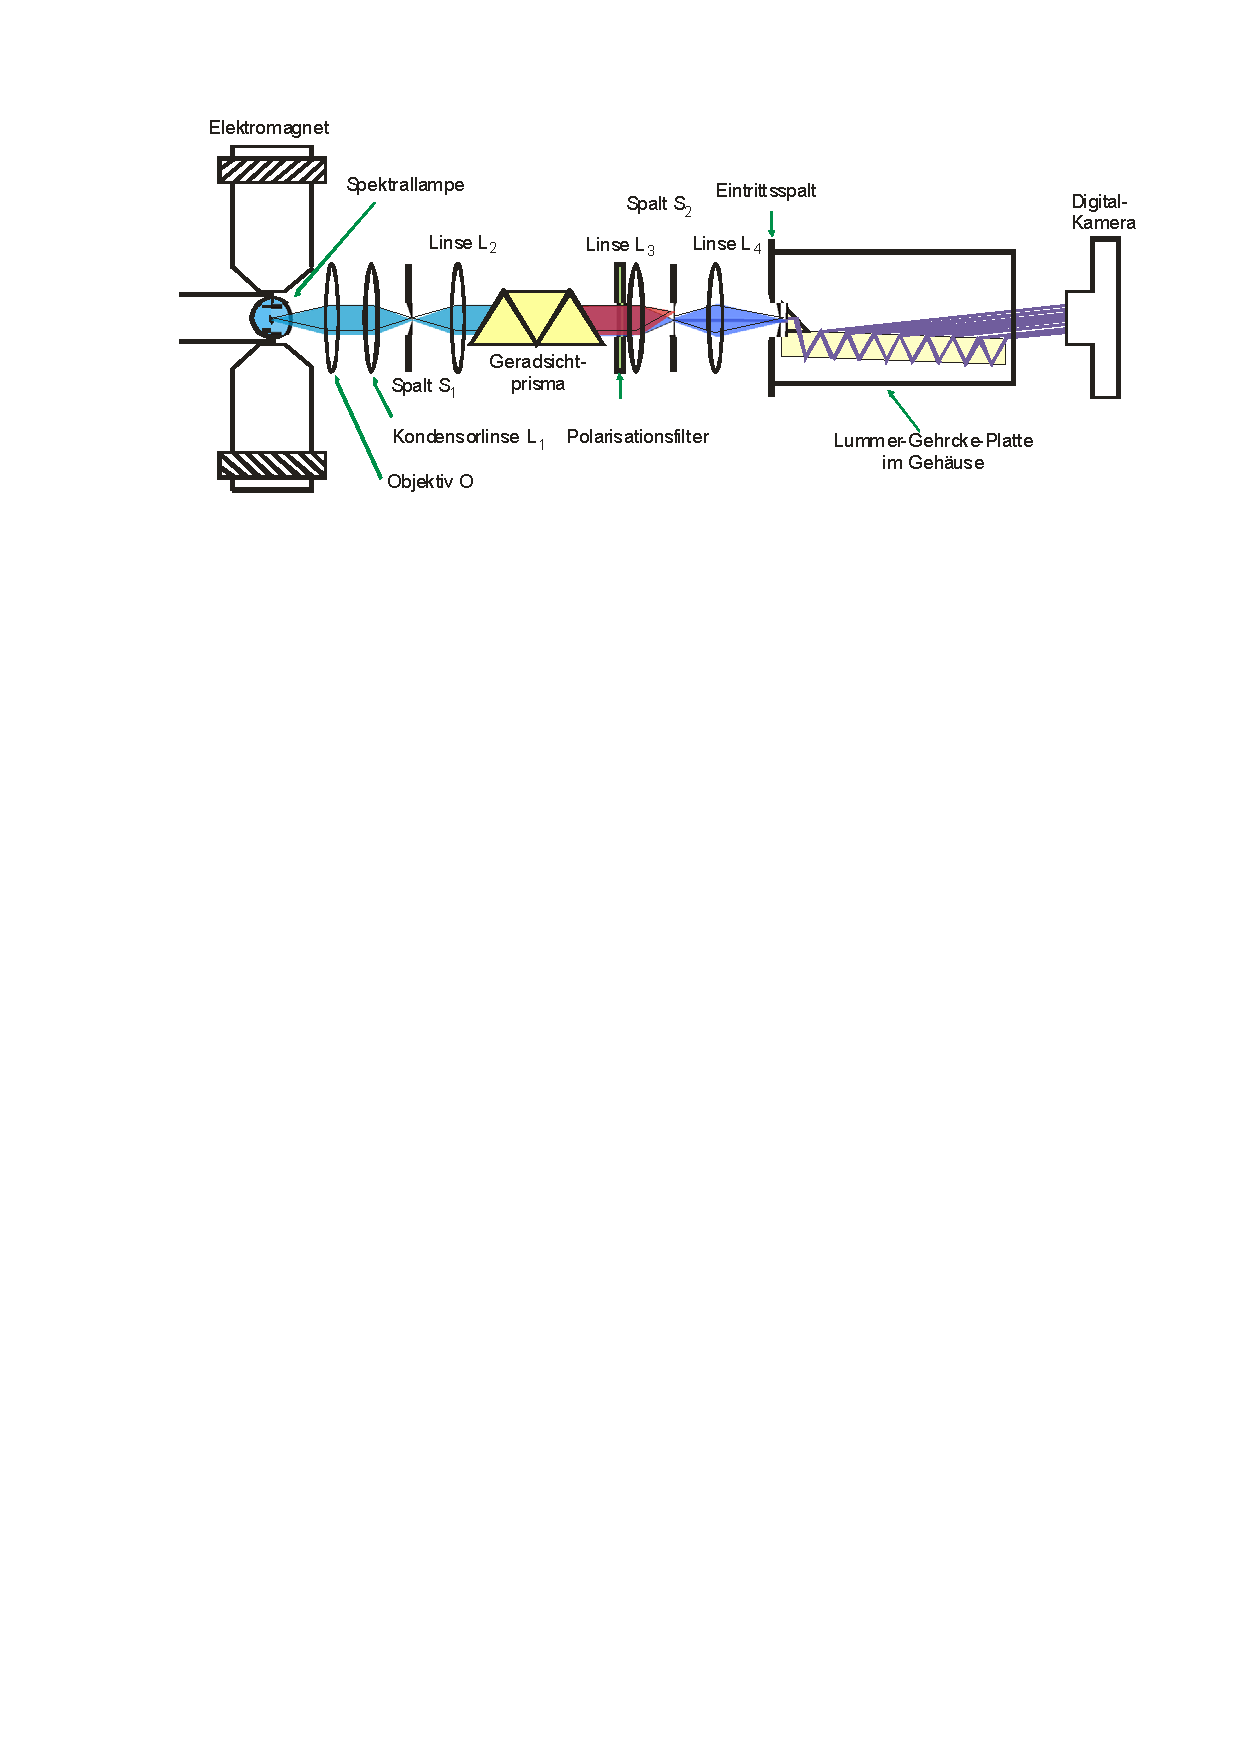
\includegraphics[width=\textwidth]{graphics/messapparatur.pdf}
    \caption{Schematischer Aufbau der Messapparatur. \cite[2]{Anleitung1}}
    \label{fig:messapparatur}
\end{figure}

Zur Untersuchung des Zeeman-Effektes wird der in Abbildung~\ref{fig:messapparatur} dargestellte
Versuchsaufbau verwendet. Dazu wird eine Cadmium-Lampe zwischen den beiden Polen des Elektromagneten positioniert.
Senkrecht zum Magnetfeld wird das emittierte Licht mit Hilfe eines Okulars, zweier Linsen und eines
Spaltes gebündelt und auf ein Geradsichtprisma gelenkt, welches die Trennung der Spektrallinien nach
ihrer Wellenlänge ermöglicht.
Dabei ist, um Intensitätsverluste zu vermeiden, darauf zu achten, dass die Abbildung des Strahlenbündels
auf das Prisma nicht größer als Selbiges ist.
Über einen nachfolgenden Polarisationsfilter kann zusätzlich die Polarisationsrichtung der zu untersuchenden
Spektrallinie eingestellt werden, wodurch zwischen den $\Delta m=0$ und $\Delta m=\pm1$ Übergängen selektiert werden kann.
Mit zwei weiteren Linsen und einem Spalt werden die Strahlen erneut gebündelt und auf eine Lummer-Gehrcke-Platte gelenkt.
\begin{figure}
    \centering
    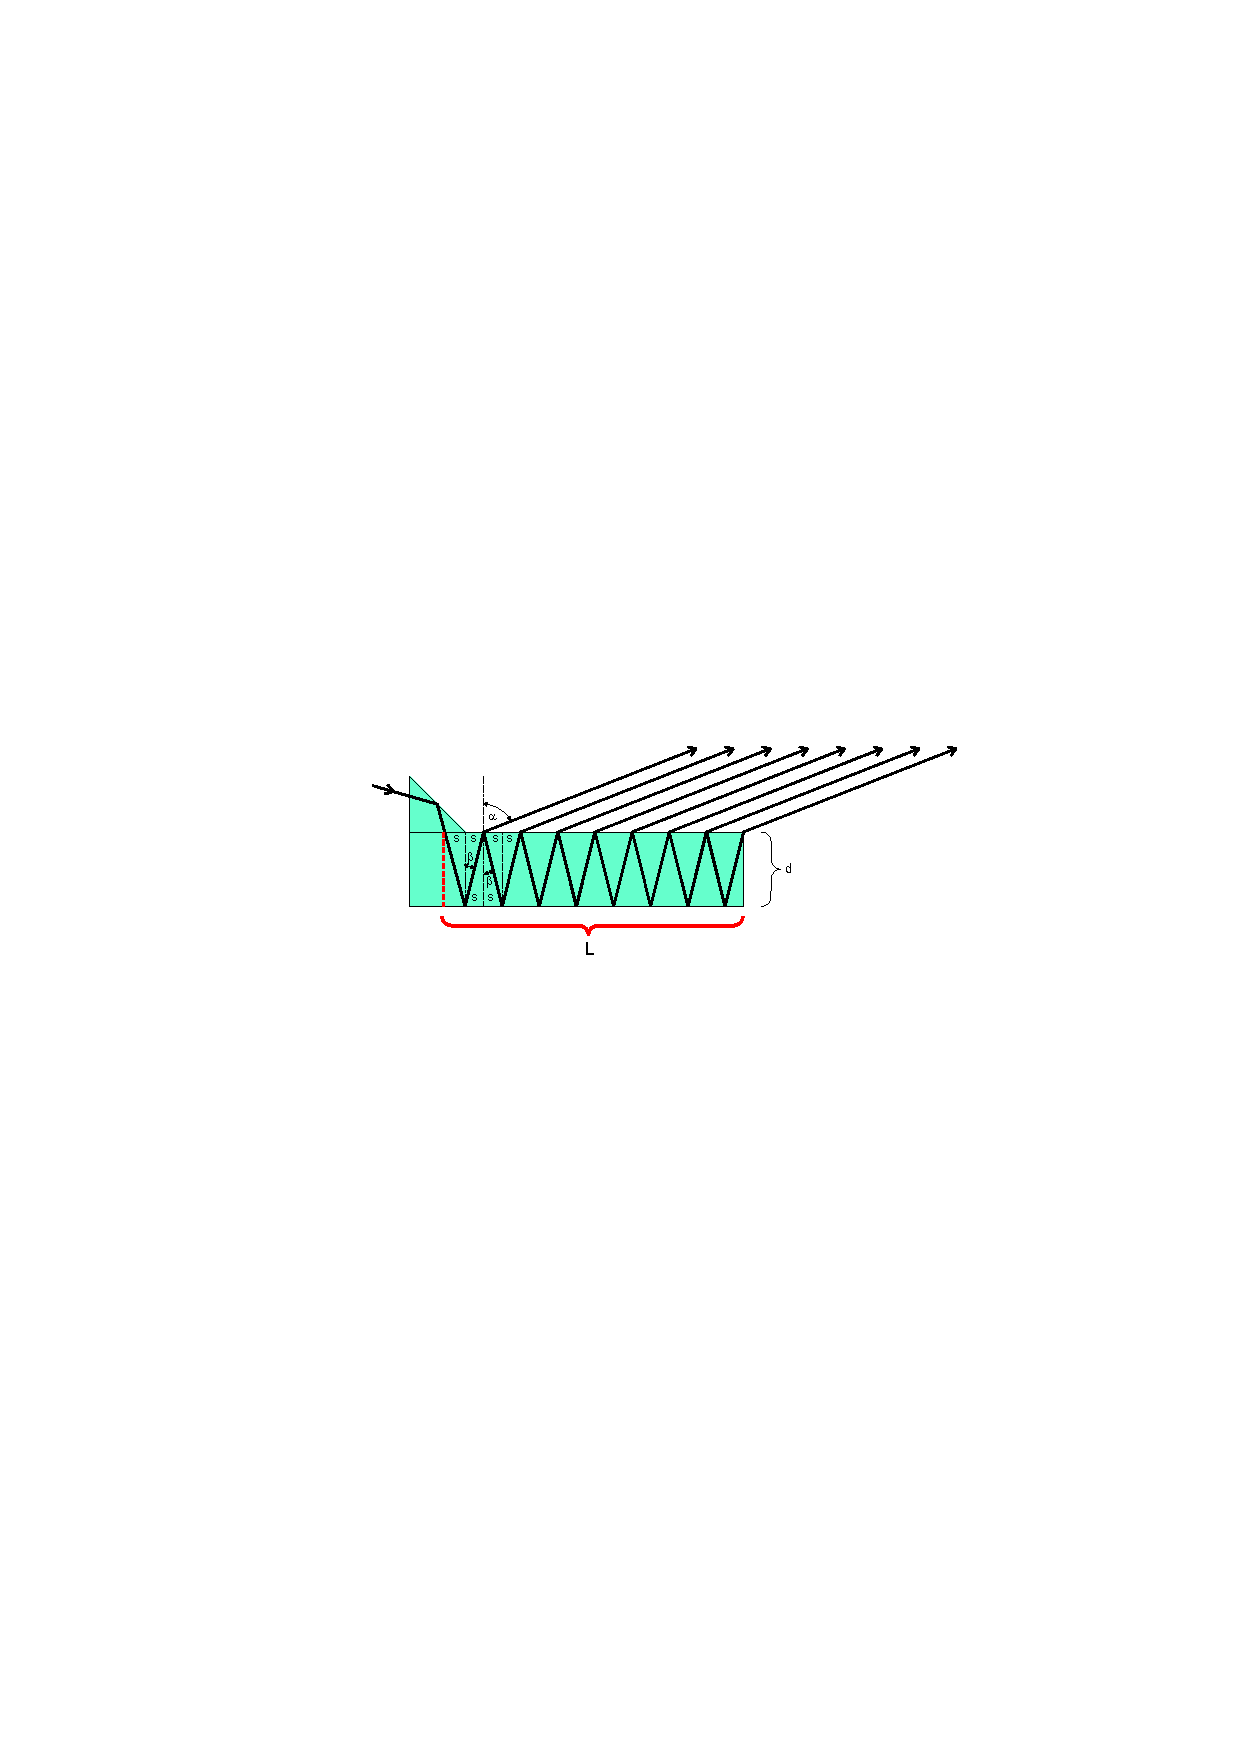
\includegraphics[width=0.7\textwidth]{graphics/lummer-gehrcke.pdf}
    \caption{Strahlengang in der Lummer-Gehrcke-Platte. \cite[2]{Anleitung1}}
    \label{fig:lummer-gehrcke}
\end{figure}
Der Strahlengang in einer solchen Platte ist schematisch in Abbildung (\ref{fig:lummer-gehrcke}) dargestellt.
Innerhalb der Platte wird das einfallende Licht mehrfach reflektiert, wobei stets ein kleiner Teil der
Strahlung aus der Platte austritt und mit anderen ausgetretenen Strahlen interferiert.
Für konstruktive Interferenz ist die Bragg-Bedingung in 1. Ordnung
\begin{equation}
    \lambda=2d\cos\theta
\end{equation}
zu erfüllen, wobei $d$ die Dicke der Platte und $\lambda$ die Wellenlänge der ausgewählten Spektrallinie ist.
Der Gangunterschied der Interferenzstreifen entspricht bei einer Lummer-Gehrcke-Platte genau der verwendeten Wellenlänge.
Das enstehende Interferenzmuster wird mit Hilfe einer am Ende des Strahlengangs befindlichen Digitalkamera aufgenommen.

\subsection{Versuchsurchführung}
Zunächst wird der verwendete Elektromagnet geeicht, dazu wird in einer Messreihe mit einer Hallsonde
das Magnetfeld in Abhängigkeit des Spulenstroms gemessen.Die Messung wird sowohl für einen ansteigenden
Strom, als auch für einen fallenden Strom durchgeführt.

Zur Untersuchung der Aufspaltung wird die rote und eine blaue Spektrallinie einer Cadmium-Spektrallampe
mit dem oben beschrieben Versuchsaufbau betrachtet. Es wird je Spektrallinie und möglicher Polarisation ein Bild
mit ausgeschaltetem und ein Bild mit eingschaltetem Magnetfeld aufgenommen. Dadurch lässt sich die Verschiebung
und Aufspaltung visualisieren.

Da eine Aufspaltung der Linien im Magnetfeld um $\delta\lambda$ auch eine Verschiebung der Interferenzstreifen um $\delta s$
bedeutet, muss auf das Dispersionsgebiet der Lummer-Gehrcke-Platte geachtet werden. Damit keine Überlagerung der Streifen
stattfindet, darf die durch die Aufspaltung bedingte Wellenlängendifferenz nicht größer als
\begin{equation}
  \label{eqn:disper}
    \Delta\lambda=\dfrac{\lambda^2}{2d}\sqrt{\dfrac{1}{n^2-1}}
\end{equation}
sein.
$n$ ist hierbei der Brechungsindex und $d$ die Dicke der Lummer-Gehrcke-Platte.
Das resultierende Auflösungsvermögen ist durch
\begin{align}
    A=\dfrac{\lambda}{\Delta\lambda}=\dfrac{L}{\lambda}(n^2-1)
\end{align}
gegeben, wobei $L$ die Länge der Platte ist.
